\documentclass[a4paper,12pt]{article}

\usepackage[top=2.5cm, bottom=2.5cm, left=3.175cm, right=3.175cm]{geometry}
\usepackage{polski}
\usepackage[utf8]{inputenc}
\usepackage{xcolor}
\usepackage{graphicx}
\usepackage{titlesec}
\usepackage{indentfirst}
\usepackage{amsmath}
\usepackage{pgfplots}
\usepackage{float}
\usepackage{minted}
\usepackage[section]{placeins}

\usetikzlibrary{positioning}

\pgfplotsset{width=7cm,compat=1.8}
\usepgfplotslibrary{patchplots}

\graphicspath{{images/}}

\numberwithin{equation}{section}

\newminted{python}{breaklines,python3,linenos,frame=single}


\tikzset{%
    every neuron/.style={
        circle,
        draw,
        minimum size=1cm
    },
    neuron input/.style={
        fill=black,
        scale=0.2,
    },
    neuron missing/.style={
        draw=none, 
        scale=3,
        text height=0.133cm,
        execute at begin node=\color{black}$\vdots$
    },
    neuron missingx/.style={
        draw=none, 
        scale=3,
        text height=0.333cm,
        execute at begin node=\color{black}$\vdots$
    },
}

\usepackage[pdftex,
            pdfauthor={Cezary Bober},
            pdftitle={Praca projektowa z przedmiotu Sztuczna Inteligencja},
            pdfsubject={Sieć neuronowa uczona algorytmem wstecznej propagacji błędu z przyśpieszeniem metodą adaptacyjnego współczynnika uczenia}]{hyperref}

\begin{document}

\pagenumbering{gobble}

\begin{titlepage}
    \includegraphics[height=1.75cm]{prz_pl.png}
    \hfill
    \includegraphics[height=1.75cm]{weii_pl.png}
    
    \centering
    \vfill
    
    {\Huge \textbf{Praca projektowa z przedmiotu Sztuczna Inteligencja} \par}
	\vspace{1.5cm}
	{\LARGE Sieć neuronowa uczona algorytmem wstecznej propagacji błędu z przyśpieszeniem metodą adaptacyjnego współczynnika uczenia \par}
	
	\vfill
    
    {\Large \textbf{Cezary Bober} \par}
    
    \vfill
    
    {\LARGE Rzeszów, 2019\par}
\end{titlepage}

\setlength{\parskip}{0.3cm}
\setlength{\parindent}{1cm}
\pagenumbering{arabic}
\setcounter{page}{2}

\tableofcontents
\pagebreak

\section{Opis projektu}
Celem projektu jest stworzenie prostej sieci neuronowej, która nauczy się rozpoznawać rodzaje wina na podstawie kilku jego parametrów. Oprócz zbudowania sieci należało także wykonać serię eksperymentów służących zbadaniu optymalnych parametrów uczenia sieci dla podanego zestawu danych.

Do stworzenia zadanej sieci neuronowej wykorzystany został język programowania \textit{Python} wraz z biblioteką \textit{Numpy} dodającą wsparcie dla m.in. wielowymiarowych macierzy.

\subsection{Zestaw danych}
Dane, na których uczyła się sieć pochodzą z zestawu \textit{Wine} \cite{dataset}. Jest to zestaw zawierający 178 rekordów opisujących wyniki analizy chemicznej 3 różnych odmian win z pewnego regionu Włoch. Każdy rekord składa się z 14 kolumn opisujących poszczególne parametry:

\begin{enumerate}
    \item Class identifier — klasa identyfikująca rodzaj wina
    \item Alcohol — procentowa zawartość alkoholu w danym winie
    \item Malic acid — zawartość kwasu jabłkowego w winie
    \item Ash — zawarość popiołu w winie
    \item Alkalinity of ash — zasadowość popiołu
    \item Magnesium — zawartość magnezu w winie
    \item Total phenols — zawartość fenoli w winie
    \item Flavanoids — zawartość flawonoidów w winie
    \item Nonflavanoid phenols — zawartość fenoli nieflawonoidowych
    \item Proanthocyanidins — zawartość proantocyjanidyn
    \item Color intensity — intensywność koloru wina
    \item Hue — barwa wina
    \item OD280/OD315 — zawartość OD280/OD315 w rozcieńczonym winie
    \item Proline — zawartość proliny w winie
\end{enumerate}

Wszystkie parametry (oprócz klasy wina, która przyjmuje wartości ze zbioru $\{1, 2, 3\}$) mają wartości ciągłe. Klasa wina jest wartością aproksymowaną przez sieć, a pozostałe parametry tworzą wektor danych wejściowych. Zestaw nie zawiera brakujących lub niepotrzebnych danych w związku z czym do nauki wykorzystany został w całości.

Przed przystąpieniem do uczenia sieci zestaw został poddany odpowiedniemu przygotowaniu. Dane zostały podzielone na część testową zawierającą 20\% wszystkich rekordów oraz część treningową zawierającą pozostałe 80\%. Rekordy są przydzielane do tych części losowo.

\begin{figure}[h]
    \vspace{0.5cm}
    \centering
    \label{fig:wine_class_chart}

    \begin{tikzpicture}
    \begin{axis}[
        width=0.9\textwidth,
        height=0.25\textheight,
        xtick = data,
        ylabel = Ilość reprezentantów,
        xlabel = Klasa wina,
        ybar,
        bar width = 30pt,
        nodes near coords,
        enlarge x limits=0.5,
        ymax = 90,
        ymin = 0
    ]
        \addplot coordinates {(1, 59) (2, 71) (3, 48)};
    \end{axis}
    \end{tikzpicture}

    \caption{Rozkład poszczególnych klas wina w zestawie}
    \vspace{0.5cm}
\end{figure}


Z analizy danych przedstawionej na rysunku \ref{fig:wine_class_chart} wynika, że poszczególne klasy wina są reprezentowane przez zbliżoną ilość rekordów dzięki czemu po rozlosowaniu wszystkich danych każda z części jest w pełni reprezentatywna.

Dodatkowo, dane wejściowe (wszytko oprócz klasy wina) zostały znormalizowane do zakresu $[-1,1]$. Do normalizacji danych wykorzystano algorytm \textit{min-max}, który pozwala znormalizować dane do wskazanego zakresu.
\begin{equation}
    X'=\frac{X-X_{min}}{X_{max}-X_{min}} \cdot (Y_{max} - Y_{min}) + Y_{min}
\end{equation}
gdzie $Y_{max}$ i $Y_{min}$ są granicami zakresu do którego chcemy znormalizować dane.


\section{Działanie sieci neuronowej}

\subsection{Działanie neuronu}
Komputerowe sieci neuronowe powstały na bazie wiedzy o działaniu systemu nerwowego istot żywych w otaczającym nas świecie. Poznanie mechanizmów działania poszczególnych neuronów jest istotne dla zrozumienia procesów przetwarzania informacji zachodzących w sieciach neuronowych.

Neuron posiada ciało, z którego wyrastają liczne wypustki łączące się z innymi neuronami. Wypustki dzielimy na liczne, cienkie \textit{dendryty} oraz oraz pojedyńczy gruby \textit{akson}. Sygnały wejściowe doprowadzane są do komórki za pośrednictwem synaps, zaś sygnał wyjściowy odprowadzany jest za pomocą aksonu. Transmisja sygnałów wewnątrz systemu nerwowego jest bardzo skomplikowanym procesem chemiczno-elektrycznym \cite{book_osowski}.


\subsection{Model neuronu sigmoidalnego}

\begin{figure}[H]
    \centering
    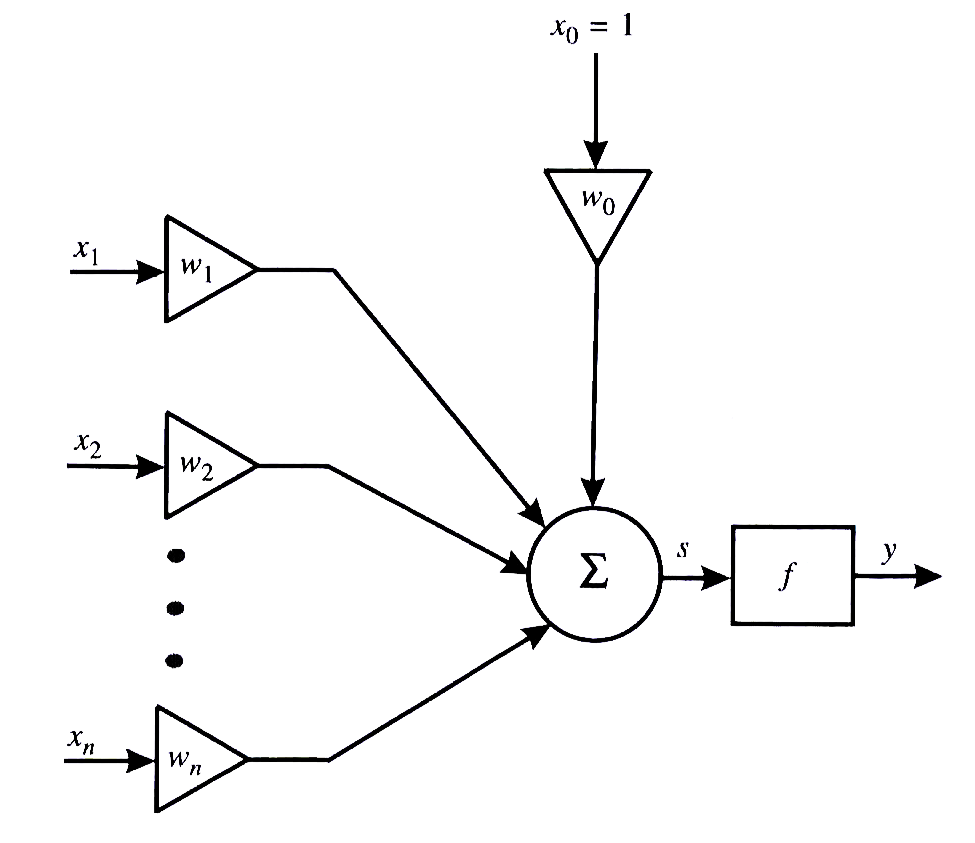
\includegraphics[width=0.7\textwidth]{sigmoid_neuron.png}
    \caption{Model neuronu (Źródło: \cite{book_rutkowski})}
    \label{fig:sigmoid_neuron}
    % \vspace{0.5cm}
\end{figure}

\noindent
$x_{1},\dots,x_{n}$ — sygnały wejściowe neuronu \vspace{0.3cm}\\
$w_{1},\dots,w_{n}$ — wagi neuronu \vspace{0.3cm}\\
$w_{0}$ — próg (bias) neuronu \vspace{0.3cm}\\
$f$ — funkcja aktywacji neuronu \vspace{0.3cm}\\
$s$ — łączne pobudzenie neuronu \vspace{0.3cm}\\
$y$ — wartość wyjściowa neuronu\\

Działanie takiego neuronu jest bardzo proste. Najpierw sygnały wejściowe $x_0,x_1,\dots,x_n$ zostają pomnożone przez odpowiadające im wagi $w_0,w_1,\dots,w_n$. Otrzymane w ten sposób wartości należy następnie zsumować. W wyniku powstaje sygnał $s$ nazywany łącznym pobudzeniem neuronu \cite{zajdel_6} odzwierciedlający działanie części liniowej neuronu. Sygnał ten jest poddawany działaniu \textit{funkcji aktywacji}. Zakładamy, że wartość sygnału $x_0$ jest równa $1$, natomiast wagę $w_0$ nazywa się progiem (ang. \textit{bias}) \cite{book_rutkowski}.

\begin{equation} \label{eq:neuron_output}
    y(t) = f(s) = f\Bigg(\sum_{i=0}^{n} w_i x_i \Bigg)
\end{equation}

\subsection{Funkcja aktywacji}
Funkcja aktywacji jest wykorzystywana do liczenia sygnału wyjściowego neuronu na podstawie jego pobudzenia. W neuronie sigmoidalnym wykorzystywana jest funkcja sigmoidalna dana wzorem:
\begin{equation} \label{eq:sigmoid_uni}
    f(x)=\frac{1}{1+e^{-\beta x}}
\end{equation}
oraz w wersji bipolarnej:
\begin{equation} \label{eq:sigmoid_bi}
    f(x)=tanh(\beta x)=\frac{e^{\beta x}-e^{-\beta x}}{e^{\beta x}+e^{-\beta x}}
    \vspace{0.3cm}
\end{equation}
Różnią się one między sobą wartościami, które zwracają. Funkcja \eqref{eq:sigmoid_uni} zwraca wartości z zakresu $[0,1]$ natomiast \eqref{eq:sigmoid_bi} z zakresu $[-1,1]$.

\begin{figure}[h]
    \vspace{0.5cm}
    \centering
    
    \begin{tikzpicture}
        \begin{axis}[
            legend pos=north west,
            axis x line=middle,
            axis y line=middle,
            y tick label style={/pgf/number format/fixed, /pgf/number format/fixed zerofill, /pgf/number format/precision=1},
            grid = major,
            width = 0.9\textwidth,
            height = 0.35\textheight,
            grid style={dashed, gray!30},
            xmin = -8,
            xmax = 8,
            ymin = -1,
            ymax = 1,
            xlabel = x,
            ylabel = y,
            % ylabel = sig(t),
            % ytick = {0.2, 0.4, 0.6, 0.8, 1.0},
            tick align = outside,
            enlarge x limits=0.1,
            enlarge y limits=0.1,
        ]
            \addplot[domain=-8:8, blue, ultra thick,samples=500] {1/(1+exp(-x))};
            \addplot[domain=-8:8, red, ultra thick,samples=500] {tanh(x)};
            
            \addlegendentry{$\frac{1}{1+e^{-x}}$}
            \addlegendentry{$tanh(x)$}
        \end{axis}
    \end{tikzpicture}

    \caption{Wykres funkcji sigmoidalnej unipolarnej (niebieski) i bipolarnej (czerwony)}
    \label{fig:sigmoid}
    \vspace{0.5cm}
\end{figure}

Zmieniając parametr $\beta$ możemy modyfikować kształt funkcji sprawiając, aby był bardziej łagodny lub stromy. Przy odpowiednim ustawieniu tego parametru funkcja sigmoidalna ma charakter progowy.

Dużą zaletą funkcji sigmoidalnej jest to, iż jest ona różniczkowalna, oraz łatwo można policzyć jej pochodną \cite{sigmoid_derivative}, która ma postać:
\begin{equation}
    f'(x)=f(x)(1-f(x))
\end{equation}
lub dla funkcji bipolarnej:
\begin{equation}
    f'(x)=(1-f^2(x))
\end{equation}


\subsection{Budowa sieci neuronowej}

Pojedyncze neurony są w stanie uczyć się rozwiązywania prostych zadań, ale już przykładowo naśladowanie funkcji XOR jest zbyt trudnym zadaniem dla pojedynczego neuronu. Z tego powodu neurony łączy się w struktury zwane warstwami. Sieć stworzona z wielu warstw jest już w stanie rozwiązywać bardziej skomplikowane zadania.

\begin{figure}[h]
    \vspace{0.5cm}
    \centering
    
    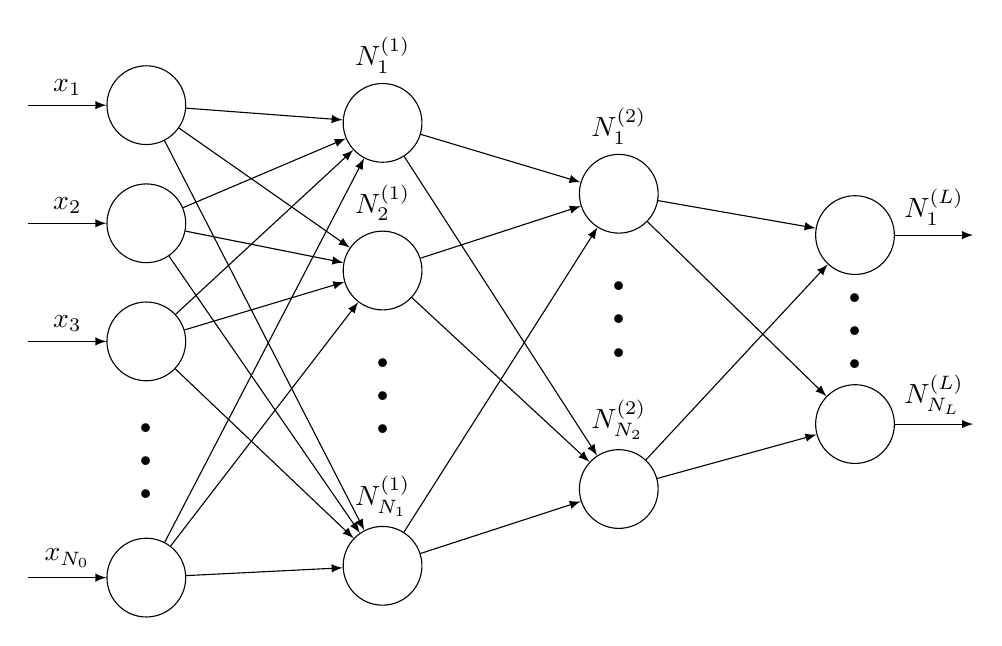
\begin{tikzpicture}[x=1.5cm, y=1.5cm, >=latex]

        \foreach \m/\l [count=\y] in {1,2,3,missingx,4}
            \node [every neuron/.try, neuron \m/.try] (input-\m) at (0,2.5-\y) {};

        \foreach \l [count=\i] in {1,2,3,{N_0}}
            \draw [<-] (input-\i) -- ++(-1,0) node [above, midway] {$x_{\l}$};

        
        \foreach \m [count=\y] in {1,2,missing,3}
            \node [every neuron/.try, neuron \m/.try ] (hidden1-\m) at (2,2.6-\y*1.25) {};
        
        \foreach \l [count=\i] in {1,2,{N_1}}
            \node [above] at (hidden1-\i.north) {$N_{\l}^{(1)}$};

        
        \foreach \m [count=\y] in {1,missing,2}
            \node [every neuron/.try, neuron \m/.try ] (hidden2-\m) at (4,2-\y*1.25) {};
        
        \foreach \l [count=\i] in {1,{N_2}}
            \node [above] at (hidden2-\i.north) {$N_{\l}^{(2)}$};
        

        \foreach \m [count=\y] in {1,missingx,2}
            \node [every neuron/.try, neuron \m/.try ] (output-\m) at (6,1.2-\y*0.8) {};
        
        \foreach \l [count=\i] in {1,{N_L}}
            \draw [->] (output-\i) -- ++(1,0) node [above, midway] {$N_{\l}^{(L)}$};
        

        \foreach \i in {1,...,4}
            \foreach \j in {1,...,3}
                \draw [->] (input-\i) -- (hidden1-\j);
        
        \foreach \i in {1,...,3}
            \foreach \j in {1,...,2}
                \draw [->] (hidden1-\i) -- (hidden2-\j);
        
        \foreach \i in {1,...,2}
            \foreach \j in {1,...,2}
                \draw [->] (hidden2-\i) -- (output-\j);
        
    \end{tikzpicture}

    \caption{Schemat sieci neuronowej wielowarstwowej}
    \label{fig:neuron_network}
    \vspace{0.5cm}
\end{figure}

Przedstawiona na rysunku \ref{fig:neuron_network} sieć składa się z warstwy wejściowej, następnie 2 warstw ukrytych oraz warstwy wyjściowej. Omawiana sieć ma $N_0$ wejść, na które podawane są sygnały $x_1(t),\dots,x_{N_0}(t)$ zapisywane w postaci wektora:
\begin{equation}
    \textbf{x}=[x_1,\dots,x_{N_0}]^T
    \hspace{1cm}
    t=1,2,\dots
\end{equation}
Każdy neuron $N_i^k$ ma przypisany wektor z wagami:
\begin{equation}
    \textbf{w}_i^{(k)}=[w_{i,0}^{(k)}, \dots, w_{i,N_{k-1}}^{(k)}]^T \hspace{1cm}
    k=1,2,\dots,L \hspace{0.5cm}
    i=1,\dots,N_k
\end{equation}
Sygnał wyjściowy \textit{i}-tego neuronu w \textit{k}-tej warstwie jest oznaczony jako:
\begin{equation}
    y_i^{(k)}=f^{(k)}(s_i^{(k)})
\end{equation}
przy czym:
\begin{equation}
    s_i^{(k)}=\sum_{j=0}^{N_{k-1}}w_{ij}^{(k)}x_j^{(k)}
\end{equation}

Sygnały wyjściowe z ostatniej warstwy są jednocześnie sygnałami wyjściowymi całej sieci. Po każdej iteracji sieci są one porównywane z \textit{sygnałami wzorcowymi} sieci \cite{book_rutkowski}
\begin{equation}
    d_1^{(L)},d_2^{(L)},\dots,d_{N_L}^{(L)}
\end{equation}

Dla poszczególnych neuronów w warstwach wyjście będzie miało postać:
\begin{equation}
    y_m^{(1)} = f^{(1)}(s_m^{(1)}) = f^{(1)} \Big( \sum_{p=1}^{N_0} x_p \cdot w_{mp}^{(1)} + w_{m0}^{(1)} \Big)
\end{equation}

\begin{equation}
\begin{aligned}
    y_j^{(2)} = f^{(2)}(s_j^{(2)}) = f^{(2)} \Big( \sum_{m=1}^{N_1} f^{(1)}(s_m^{(1)}) \cdot w_{jm}^{(2)} + w_{j0}^{(2)} \Big) = \\
    = f^{(2)} \Big( \sum_{m=1}^{N_1} f^{(1)} \Big(\sum_{p=1}^{N_0} x_p \cdot w_{mp}^{(1)} + w_{m0}^{(1)} \Big) \cdot w_{jm}^{(2)} + w_{j0}^{(2)} \Big)
\end{aligned}
\end{equation}

\begin{equation}
\begin{aligned}
    y_i^{(3)} = f^{(3)}(s_i^{(3)}) = f^{(3)} \Big( \sum_{j=1}^{N_2} f^{(2)}(s_j^{(2)}) \cdot w_{ij}^{(3)} + w_{i0}^{(3)} \Big) = \\
    f^{(3)} \Big( \sum_{j=1}^{N_2} f^{(2)} \Big( \sum_{m=1}^{N_1} f^{(1)} \Big(\sum_{p=1}^{N_0} x_p \cdot w_{mp}^{(1)} + w_{m0}^{(1)} \Big) \cdot w_{jm}^{(2)} + w_{j0}^{(2)} \Big) \cdot w_{ij}^{(3)} + w_{i0}^{(3)} \Big)
\end{aligned}
\end{equation}

Błąd sieci liczymy jako:
\begin{equation}
    Q = \sum_{m=1}^{N_L}{\Big(d_m^{(L)}-y_m^{(L)}\Big)}^2
\end{equation}

\subsection{Wsteczna propagacja błędu}
Podczas uczenia sieci jednowarstwowych w łatwy sposób można zdefiniować błąd na wyjściu sieci ponieważ znamy wartość otrzymaną oraz wartość, która powinna być na wyjściu. Problem pojawia się jednak przy tworzeniu sieci wielowarstwowych. Nie znamy bowiem wartości jakie powinny być na wyjściu poszczególnych neuronów w warstwach ukrytych. W celu rozwiązania tego problemu wymyślono \textit{metodę wstecznej propagacji błędów} \cite{book_rutkowski}.

W metodzie tej do określania błędów na poszczególnych warstwach wykorzystuje się gradienty. Cały proces zaczyna się od końca sieci, stąd nazwa \textit{wsteczna propagacja}. Do obliczenia zmiany $\Delta w_{ij}$ musimy policzyć pochodną cząstkową z funkcji kosztu względem wagi $w_{ij}$.
\begin{equation}
    \label{eq:delta_w}
    \Delta w_{ij} = -\eta \frac{\partial Q}{\partial w_{ij}}
\end{equation}
gdzie $\eta$ to współczynnik uczenia sieci. Nie wiemy jak bezpośrednio policzyć taką pochodną dlatego musimy rozpisać ją tak, abyśmy otrzymali składniki, które umiemy policzyć.

Przykładowo dla przedstawionej na rysunku \ref{fig:neuron_network} sieci, aby obliczyć zmianę wag dla warstwy wyjściowej rozpiszemy \cite{zajdel_9}:
\begin{equation}
    \label{eq:gradient1}
    \frac{\partial Q}{\partial w^{(L)}_{ij}} = \frac{\partial Q}{\partial f^{(L)}} \frac{\partial f^{(L)}(s_i^{(L)})}{\partial s^{(L)}_i} \frac{\partial s^{(L)}_i}{\partial w^{(L)}_{ij}} 
\end{equation}
Możemy zauważyć, że
\begin{equation}
    \frac{\partial Q}{\partial f^{(L)}} = 2(y_i^{(L)} - d^{(L)}_i)
\end{equation}
oraz
\begin{equation}
    \frac{\partial s^{(L)}_i}{\partial w^{(L)}_{ij}} = y^{(2)}_j
\end{equation}
W związku z czym możemy równanie \ref{eq:gradient1} zapisać jako:
\begin{equation}
    \frac{\partial Q}{\partial w^{(L)}_{ij}} = 2(y_i^{(L)} - d^{(L)}_i) \frac{\partial f^{(L)}(s_i^{(L)})}{\partial s^{(L)}_i} y^{(2)}_j
\end{equation}

\noindent Następnie postępujemy w analogiczny sposób dla warstwy 2:
\begin{equation}
    \frac{\partial Q}{\partial w_{jm}^{(2)}} = \frac{\partial Q}{\partial f^{(L)}} \frac{\partial f^{(L)}(s_i^{(L)})}{\partial s^{(L)}_i} \frac{\partial s^{(L)}_i}{\partial f^{(2)}} \frac{\partial f^{(2)}(s_j^{(2)})}{\partial s^{(2)}_j} \frac{\partial s_j^{(2)}}{\partial  w_{jm}^{(2)}}
\end{equation}

\begin{equation}
    \frac{\partial Q}{\partial w^{(2)}_{jm}} = \sum_{i=1}^{N_L} 2(y_i^{(L)} - d^{(L)}_i) \frac{\partial f^{(L)}(s_i^{(L)})}{\partial s^{(L)}_i} w^{(L)}_{ij} \frac{\partial f^{(2)}(s_j^{(2)})}{\partial s^{(2)}_j} y^{(1)}_m
\end{equation}

\noindent oraz dla warstwy 1:
\begin{equation}
    \frac{\partial Q}{\partial w_{mp}^{(1)}} = \frac{\partial Q}{\partial f^{(L)}} \frac{\partial f^{(L)}(s_i^{(L)})}{\partial s^{(L)}_i} \frac{\partial s^{(L)}_i}{\partial f^{(2)}} \frac{\partial f^{(2)}(s_j^{(2)})}{\partial s^{(2)}_j} \frac{\partial s_j^{(2)}}{\partial  f^{(1)}} \frac{\partial f^{(1)}(s_m^{(1)})}{\partial s_m^{(1)}} \frac{\partial s_m^{(1)}}{\partial w_{mp}^{(1)}}
\end{equation}

\begin{equation}
    \frac{\partial Q}{\partial w_{mp}^{(1)}} = \sum_{i=1}^{N_L} 2(y_i^{(L)} - d^{(L)}_i) \frac{\partial f^{(L)}(s_i^{(L)})}{\partial s^{(L)}_i} \sum_{j=1}^{N_2} w^{(L)}_{ij} \frac{\partial f^{(2)}(s_j^{(2)})}{\partial s^{(2)}_j} w^{(2)}_{jm} \frac{\partial f^{(1)}(s_m^{(1)})}{\partial s_m^{(1)}} x_p
\end{equation}

W ten sposób możemy policzyć zmianę wag dla dowolnie głębokiej sieci neuronowej.

W książce \cite{book_rutkowski} przedstawiona została pewna modyfikacja tych wzorów, dzięki której implementacja tego algorytmu w kodzie jest łatwiejsza. Podczas liczenia zmiany wagi wprowadzany jest $\varepsilon_i^{(k)}$ w postaci:
\begin{equation}
    \label{eq:epsilon}
    \varepsilon_i^{(k)}=\sum_{m=1}^{N_{k+1}}\delta^{(k+1)}_m w_{mi}^{(k+1)} \hspace{1cm} k=1,\dots,L-1
\end{equation}
następnie korzystając z obliczonej w \ref{eq:epsilon} wartości liczymy $\delta_i^{(k)}$:
\begin{equation}
    \delta_i^{(k)} = \varepsilon_i^{(k)} f'(s_i^{(k)})
\end{equation}
Zmiana wagi jest wtedy wyrażona jako:
\begin{equation}
    \Delta w_{ij}^{(k)} = 2 \eta \delta_i^{(k)} x_j^{(k)}
\end{equation}
Od wzoru \ref{eq:delta_w} różni się podstawieniem:
\begin{equation}
    \delta_i^{(k)} = -\frac{1}{2} \frac{\partial Q}{\partial s_i^{(k)}}
\end{equation}
\begin{equation}
    \frac{\partial Q}{\partial w_{ij}^{(k)}} = -2 \delta_i^{(k)} x_j^{(k)}
\end{equation}


\subsection{Adaptacyjny współczynnik uczenia}
\label{subsec:adaptive_lr}
W trakcie uczenia się sieci ważne jest aby współczynnik uczenia nie był zbyt duży aby nie pominąć minimum funkcji kosztu. Jednakże przy zbyt niskim współczynniku proces uczenia może trwać bardzo długo. Rozwiązaniem tego problemu jest \textit{adaptacyjny współczynnik uczenia}.

Podczas uczenia sieci należy obserwować błąd na wyjściu sieci. Jeżeli błąd w stosunku do poprzedniej chwili czasu wzrósł w sposób istotny
\begin{equation}
    err(t+1) > err\_ratio \cdot err(t)
\end{equation}
to nowo wyliczone wagi oraz biasy zostają odrzucone, a współczynnik uczenia zostaje pomniejszony o odpowiednią wartość:
\begin{equation}
    \eta(t+1) = \eta(t) \cdot lr\_dec
\end{equation}
Natomiast w przypadku gdy błąd zmalał w stosunku do poprzedniej iteracji
\begin{equation}
    err(t+1) < err(t)
\end{equation}
to współczynnik uczenia jest zwiększany
\begin{equation}
    \eta(t+1) = \eta(t) \cdot lr\_inc
\end{equation}
W innych przypadkach współczynnik uczenia zostaje bez zmian.

Dzięki zastosowaniu tej metody sieć będzie \textit{przyspieszała} i \textit{zwalniała} w odpowiednich momentach dzięki czemu proces nauczania sieci będzie krótszy.

Przykładowo w programie \textit{MATLAB} standardowo przyjęte są wartości:\\
$err\_ratio=1.04$, $lr\_dec=0.7$ oraz $lr\_inc=1.05$. W rezultacie, jeżeli błąd zwiększy się o 4\% to współczynnik uczenia zostanie zmniejszony o 30\%, a gdy błąd zmniejszy się to współczynnik uczenia wzrośnie o 5\% \cite{mathworks_adaptive}.


\section{Realizacja sieci w języku Python}
Opisana powyżej sieć została zaimplementowana w języku \textit{Python}. Oprócz standardowej biblioteki program wykorzystuje pakiet \textit{Numpy} ułatwiający pracę na macierzach oraz bibliotekę \textit{Pyplot} do tworzenia wykresów. Całość kodu (oprócz funkcji do inicjalizacji wag i biasów) została napisana \textit{od zera}.

\subsection{Kod programu}
\noindent
\textbf{Uwaga:} Z poniższego kodu wycięte zostały fragmenty nie mające związku z prezentowanym algorytmem tj. wypisywanie tekstu do konsoli, tworzenie wykresu, zapisywanie modelu itp. w celu zachowania przejrzystości kodu.

\begin{pythoncode}
def normalize(data, min_v=-1, max_v=1):
    for i in range(data.shape[0]):
        data[i] = ((data[i] - data[i].min()) / (data[i].max() - data[i].min())) * (max_v - min_v) + min_v
    return data
\end{pythoncode}

\noindent Funkcja \mintinline{python}{normalize()} służy do normalizacji danych w macierzy dwuwymiarowej do wybranego zakresu.


\begin{pythoncode}
def load_wine(test_count=20, sort_training=False):
    with open('wine.csv') as f:
        wines = np.array([list(map(float, x.strip().split(','))) for x in f])
        np.random.shuffle(wines)
        a = int((wines.shape[0] / 100) * test_count)
        wines[:, 1:] = normalize(wines[:, 1:].T).T

        test_wines = wines[:a]
        test_wines = test_wines[test_wines[:,0].argsort()]
        testing_data = (test_wines[:, 1:], test_wines[:, 0])

        wines = wines[a:]
        
        if sort_training:
            wines = wines[wines[:,0].argsort()]
        
        learning_data = (wines[:, 1:], wines[:, 0])
    
    return (learning_data, testing_data)
\end{pythoncode}

\noindent Wczytywanie danych odbywa się za pomocą funkcji \mintinline{python}{load_wine()}. Na początku dane są ładowane z pliku pobranego ze strony \cite{dataset}. Następnie zostają one wczytane do tablicy jako liczby zmiennoprzecinkowe. Po wczytaniu kolejność rekordów jest mieszana, a zestaw jest normalizowany do zakresu $[-1, 1]$ korzystając z funkcji \mintinline{python}{normalize()}. Po normalizacji zestaw jest dzielony na dwie części (domyślnie na 20\% i 80\%). Jeżeli zmienna \mintinline{python}{sort_training} jest ustawiona na \mintinline{python}{True} to część treningowa danych jest sortowana według klasy.


\begin{pythoncode}
class NeuralNetwork:
    def __init__(self, lr, epochs, layers, err_ratio, lr_inc, lr_dec, goal):
        self.lr = lr
        self.epochs = epochs
        self.layers = layers
        self.err_ratio = err_ratio
        self.lr_inc = lr_inc
        self.lr_dec = lr_dec
        self.goal = goal
        self.weights = None
\end{pythoncode}

\noindent Sieć zaimplementowana jest jako klasa \mintinline{python}{NeuralNetwork}. Podczas jej inicjalizacji odpowiednie pola ustawiane są na wartości przekazane w konstruktorze.


\begin{pythoncode}
def feed_training_data(self, P, T):
    self.P = P
    self.T = T

def feed_test_data(self, P, T):
    self.test_P = P
    self.test_T = T
\end{pythoncode}

\noindent Funkcje \mintinline{python}{feed_training_data()} oraz \mintinline{python}{feed_test_data()} inicjalizują dane wykorzystywane przez sieć do uczenia i testowania.


\begin{pythoncode}
def activation(self, x, derivative=False, beta=1):
    return np.tanh(beta * x) if not derivative else 1 - np.tanh(beta * x)**2

def linear(self, x, derivative=False):
    return 1 if derivative else x
\end{pythoncode}

\noindent Funkcja \mintinline{python}{activation()} w zależności od podanych parametrów zwraca obliczoną wartość funkcji sigmoidalnej bipolarnej dla danego argumentu lub wartość pochodnej. Funkcja \mintinline{python}{linear()} działa na tej samej zasadzie lecz dla funkcji liniowej.


\label{code:initnw}
\begin{pythoncode}
def initnw(layer_size, input_size):
    beta = 0.7 * (layer_size ** (1.0 / input_size))
    w_rand = np.random.rand(layer_size, input_size) * 2 - 1
    w_rand = np.sqrt(1.0 / np.square(w_rand).sum(axis=1).reshape(layer_size, 1)) * w_rand

    w = beta * w_rand
    b = beta * np.linspace(-1, 1, layer_size) * np.sign(w[:, 0])

    return w, b
\end{pythoncode}

\noindent Funkcja \mintinline{python}{initnw()} jest zmodyfikowaną wersją kodu z biblioteki \textit{NeuroLab} \cite{initnw}. Służy ona do generowania współczynników wagowych oraz biasów zgodnie z postulatami zawartymi w \cite{nguyen_widrow}. Na początku obliczany jest współczynnik szerokości przedziału, następnie wagi inicjowane są jako liczby z przedziału [-1, 1]. W kolejnym kroku liczona jest norma Euklidesowa, przez którą wraz z obliczonym współczynnikiem zostają przemnożone wagi. Dzięki zastosowaniu tego algorytmu wagi dalej pozostają w pewnym stopniu losowe, ale są równomiernie rozłożone względem danych wejściowych.


\begin{pythoncode}
def init_weights_and_biases(self):
    self.weights, self.biases = [], []
    sizes = [self.P.shape[1], *self.layers]

    for i in range(1, len(sizes)):
        w, b = initnw(sizes[i], sizes[i-1])
        self.weights.append(w)
        self.biases.append(b)

    self.weights.append(np.random.rand(1, sizes[-1]))
    self.biases.append(np.random.rand(1))
\end{pythoncode}

\noindent W funkcji \mintinline{python}{init_weights_and_biases()} inicjalizowane są wagi generowane przy użyciu funkcji \mintinline{python}{initnw()}. Jedynie w ostatniej (wyjściowej) warstwie generowane dane korzystają z klasycznej funkcji \mintinline{python}{rand()}.

\noindent Zmienna \mintinline{python}{self.weights} jest listą zawierającą tyle elementów ile warstw ma sieć (nie licząc warstwy wejściowej). W każdym z nich znajduje się tablica o rozmiarze $M \times N$ gdzie $M$ oznacza liczbę neuronów w warstwie, a $N$ liczbę neuronów w warstwie poprzedzającej.

\noindent \mintinline{python}{self.biases} jest natomiast listą zawierającą tyle elementów ile warstw ma sieć, gdzie każdy element jest tablicą $M$-elementową, w której $M$ oznacza liczbę neuronów w warstwie.


\begin{pythoncode}
def forward(self, x):
    y, sum_inputs = [x], []
    for i in range(len(self.layers) + 1):
        f = self.linear if i == len(self.layers) else self.activation
        s = [np.dot(y[i], w) for w in self.weights[i]] + self.biases[i]
        y.append(f(s))
        sum_inputs.append(s)
    return y, sum_inputs
\end{pythoncode}

\noindent Przejście do przodu przez całą sieć realizowane jest przez funkcję \mintinline{python}{forward()}. Wewnątrz pętli, dla każdej warstwy wybierany jest rodzaj używanej funkcji aktywacji, następnie liczone jest całkowite pobudzenie neuronów korzystając z funkcji do liczenia iloczynu skalarnego macierzy. Funkcja na koniec oblicza wyjścia neuronów, zwraca listę zawierającą wyjścia neuronów oraz listę ze wszystkimi pobudzeniami.


\begin{pythoncode}
def predict(self, x):
    return self.forward(x)[0][-1][0]
\end{pythoncode}

\noindent Funkcja \mintinline{python}{predict()} przyjmuje tablicę z danymi dotyczącymi jednego wina i zwraca jedną liczbę, którą jest wyjście z sieci.


\begin{pythoncode}
def test(self, P, T):
    prediction = [self.predict(x) for x in P]
    error = np.array([d - y for y, d in zip(prediction, T)])
    cost = (error**2).sum()
    pk = int(((error**2) < 0.25).sum() / len(error) * 100)
    return prediction, cost, pk
\end{pythoncode}

\noindent Funkcja \mintinline{python}{test()} służy do przetestowania sieci na podanych w argumentach danych. Przeprowadzany jest test, obliczany koszt oraz poprawność klasyfikacji wyrażona w procentach. Na koniec wyjścia z sieci oraz obliczone wskaźniki są zwracane.


\begin{pythoncode}
def errors(self, d, y, sum_inputs):
    delta = [d - y[-1]]
    for k in range(len(self.layers), 0, -1):
        epsilon = [np.dot(delta[0], w) for w in self.weights[k].T]
        delta.insert(0, np.array(epsilon * self.activation(sum_inputs[k-1], True)))
    return delta
\end{pythoncode}

\noindent Funkcja \mintinline{python}{errors()} odpowiedzialna jest za obliczenie odpowiednich wartości do aktualizacji wag wykorzystując metodę wstecznej propagacji błędów. W każdej iteracji pętli (która przechodzi od warstwy wyjściowej poprzez wszystkie warstwy ukryte) obliczany jest błąd warstwy, który dla pojedynczego neuronu ma postać jak w \ref{eq:epsilon} oraz $\delta_i^{(k)}$. Na koniec obliczone delty są zwracane.
    
\begin{pythoncode}
def update_weights_and_biases(self, delta, x):
    for i in range(len(self.layers) + 1):
        for j in range(len(self.weights[i])):
            factor = 2 * self.lr * delta[i][j]
            self.weights[i][j] += (factor * x[i])
            self.biases[i][j] += (factor * 1)
\end{pythoncode}

\noindent W funkcji \mintinline{python}{update_weights_and_biases()} następuje aktualizacja wag oraz biasów neuronów. Wykorzystywana jest $\delta_i^{(k)}$ policzona w funkcji \mintinline{python}{errors()}.

\begin{pythoncode}
def update_learning_rate(self, cost):
    if len(self.costs) > 1:
        if cost > self.costs[-1] * self.err_ratio:
            self.lr = max(1e-10, self.lr * self.lr_dec)
            self.weights = self.last_weights
            self.biases = self.last_biases
            return False
        elif cost < self.costs[-1]:
            self.lr = min(1 - 1e-10, self.lr * self.lr_inc)
    return True
\end{pythoncode}

\noindent Algorytm adaptacyjnego współczynnika uczenia opisany w sekcji \ref{subsec:adaptive_lr} jest realizowany za pomocą funkcji \mintinline{python}{update_learning_rate()}. Użyte funkcje \mintinline{python}{max()} i \mintinline{python}{min()} służą zabezpieczeniu aby współczynnik uczenia nie wyszedł poza zakres (0, 1).


\begin{pythoncode}
def start_learning(self):
    self.init_weights_and_biases()
    self.costs, self.pks = [], []
    self.last_weights, self.last_biases = [], []

    for epoch in range(self.epochs):
        for x, d in zip(self.P, self.T):
            y, sum_inputs = self.forward(x)
            delta = self.errors(d, y, sum_inputs)
            self.update_weights_and_biases(delta, y)

        prediction, cost, pk = self.test(self.test_P, self.test_T)
        
        if self.update_learning_rate(cost):
            self.costs.append(cost)
            self.pks.append(pk)
        else:
            self.costs.append(self.costs[-1])
            self.pks.append(self.pks[-1])

        if cost <= self.goal or pk == 100:
            break

        self.last_weights = self.weights
        self.last_biases = self.biases

    return self.costs
\end{pythoncode}

\noindent Metoda \mintinline{python}{start_learning()} rozpoczyna proces uczenia się sieci. Na początku inicjowane są wagi i biasy, następnie uruchamiana jest pętla wykonująca się przez zadeklarowaną ilość epok oraz pętla podająca kolejne rekordy danych.

\noindent W każdej iteracji liczone jest wyjście sieci oraz łączne pobudzenie neuronów, następnie liczone są błędy poszczególnych neuronów po czym aktualizowane są wagi oraz biasy. Podejście to nosi nazwę \textit{przyrostowego uaktualniania wag} \cite{book_rutkowski}.

\noindent Po przejściu każdej epoki sieć jest testowana a wyniki zapisywane w celu późniejszego ich przedstawienia na wykresie. Następnie następuje aktualizacja współczynnika nauczania. Jeżeli koszt spadł poniżej zadanego progu lub sieć osiągnęła 100\% poprawności klasyfikacji to następuje przerwanie procesu nauczania w przeciwnym razie rozpoczyna się kolejna epoka.



\section{Eksperymenty}

W ramach tej części projektu zbadane zostało jak pewne zmiany domyślnych wartości parametrów sieci wpływają na poprawę lub pogorszenie się procesu uczenia sieci.

\subsection{Wpływ sposobu inicjalizacji wag na szybkość uczenia sieci}

W tym eksperymencie sprawdzone zostało jaki wpływ na szybkość uczenia sieci ma użycie dwóch różnych metod inicjalizacji wag. Porównane zostało generowanie wag w sposób losowy, oraz za pomocą algorytmu \textit{Nguyen'a-Widrow'a}, którego kod znajduje się w sekcji \ref{code:initnw}. Do przeprowadzenia testu został wykorzystany następujący program
\begin{pythoncode}
learning_data, testing_data = load_wine()
net = nn.NeuralNetwork(0.01, 1000, [10, 8], 1.04, 1.05, 0.7, 0.20)
net.feed_training_data(*learning_data)
net.feed_test_data(*testing_data)
costs = net.start_learning()
\end{pythoncode}
W teście sieć o 2 warstwach ukrytych o ilości neuronów $S_1=10$ i $S_2=8$ uczyła się przez $1000$ epok.

Dodatkowo przy testowaniu losowych wag została zmodyfikowana funkcja \mintinline{python}{init_weights_and_biases()} w sposób następujący:
\begin{pythoncode}
def init_weights_and_biases(self):
    self.weights, self.biases = [], []
    sizes = [self.P.shape[1], *self.layers, 1]

    for i in range(1, len(sizes)):
        self.weights.append(np.random.rand(sizes[i], sizes[i-1]))
        self.biases.append(np.random.rand(sizes[i]))
\end{pythoncode}

\noindent Zebrane wyniki eksperymentu przedstawiono na rysuku \ref{fig:exp_1}.

\begin{figure}[!htpb]
    \centering

    \begin{tikzpicture}
        \begin{axis}[
            width=\textwidth,
            height=0.6\textwidth,
            xlabel={Epoki},
            ylabel={Wartość funkcji kosztu},
            every axis plot/.append style={ultra thick},
            no markers,
        ]
            \addplot table[mark=none] {data/exp_1_1_rand.dat};
            \addplot table[mark=none] {data/exp_1_1_nw.dat};
            \legend{Wagi losowe, Alg. Nguyen'a-Widrow'a}
        \end{axis}
    \end{tikzpicture}

    \caption{Poziom nauczenia sieci po 1000 epokach dla dwóch metod inicjalizacji wag}
    \label{fig:exp_1}
\end{figure}

Eksperyment pokazał, że dla wag w pełni losowych początkowy koszt jest prawie 6-krotnie wyższy niż dla wag inicjalizowanych algorytmem \textit{Nguyen'a-Widrow'a}. Dodatkowo funkcja kosztu dużo szybciej spada do niewielkich wartości.

\begin{figure}[!htpb]
    \centering

    \begin{tikzpicture}
        \begin{axis}[
            width=\textwidth,
            height=0.6\textwidth,
            xlabel={Epoki},
            ylabel={Wartość funkcji kosztu},
            every axis plot/.append style={ultra thick},
            ymax=0.5,
            no markers,
        ]
            \addplot table[mark=none] {data/exp_1_1_rand.dat};
            \addplot table[mark=none] {data/exp_1_1_nw.dat};
            \legend{Wagi losowe, Alg. Nguyena-Widrowa}
        \end{axis}
    \end{tikzpicture}

    \caption{Zbliżenie na wykres kosztu przy użyciu dwóch metod inicjalizacji wag}
    \label{fig:exp_1_zoom}
\end{figure}

Na zbliżeniu widać także, że koszt maleje bez dużych skoków jak to było przy wagach losowych. W związku z tym do kolejnych eksperymentów algorytm ten będzie wykorzystywany przy inicjalizowaniu wag.

\FloatBarrier
\subsection{Wpływ rozkładu klas w danych wejściowych na szybkość uczenia}

W tym eksperymecnie zestawione zostały ze sobą dwie wersje danych wejściowych — posortowane według klas, oraz przetasowane w losowej kolejności. Do przeprowadzenia eksperymentu użyto kodu:

\begin{pythoncode}
learning_data, testing_data = load_wine()
net = nn.NeuralNetwork(0.01, 20, [10, 8], 1.04, 1.05, 0.7, 0.20)
net.feed_training_data(*learning_data)
net.feed_test_data(*testing_data)
net.start_learning()
prediction, cost, pk = net.test(*testing_data)
\end{pythoncode}
Dodatkowo przy testowaniu danych posortowanych funkcja \mintinline{python}{load_wine()} została użyta z flagą \mintinline{python}{sort_training}, która odpowiada za posortowanie danych.

W pierwszej części eksperymentu zatrzymano sieć po 1 epoce aby zobaczyć jak prezentuje się poziom nauczenia sieci na samym początku.\\

\begin{figure}[h]
    \centering

    \begin{tikzpicture}
        \begin{axis}[
            width=\textwidth,
            height=0.6\textwidth,
            xlabel={Wzorzec},
            ylabel={Klasa wina},
            every axis plot/.append style={ultra thick},
            no markers,
            legend pos=south east,
        ]
            \addplot table[mark=none] {data/exp_2_sort_pred.dat};
            \addplot table[mark=none] {data/exp_2_sort_target.dat};
            \legend{Wyjście sieci, Wartości oczekiwane}
        \end{axis}
    \end{tikzpicture}

    \caption{Klasyfikacja wina przez sieć po 1 epoce dla danych posortowanych}
    \label{fig:exp_2_sort}
    \vspace{0.5cm}
\end{figure}

\begin{figure}[H]
    \centering

    \begin{tikzpicture}
        \begin{axis}[
            width=\textwidth,
            height=0.6\textwidth,
            xlabel={Wzorzec},
            ylabel={Klasa wina},
            every axis plot/.append style={ultra thick},
            no markers,
            legend pos=south east,
        ]
            \addplot table[mark=none] {data/exp_2_shuffle_pred.dat};
            \addplot table[mark=none] {data/exp_2_shuffle_target.dat};
            \legend{Wyjście sieci, Wartości oczekiwane}
        \end{axis}
    \end{tikzpicture}

    \caption{Klasyfikacja wina przez sieć po 1 epoce dla danych nieposortowanych}
    \label{fig:exp_2_shuffle}
\end{figure}

Z wykresów \ref{fig:exp_2_sort} i \ref{fig:exp_2_shuffle} wyraźnie widać, że już po 1 epoce sieć z danymi nieposortowanymi radziła sobie dużo lepiej, Poszczególne predykcje sieci były o wiele bliższe wartościom oczekiwanym niż jak to było przy danych posortowanych według klas.

\begin{figure}[H]
    \centering

    \begin{tikzpicture}
        \begin{axis}[
            width=\textwidth,
            height=0.6\textwidth,
            xlabel={Wzorzec},
            ylabel={Klasa wina},
            every axis plot/.append style={ultra thick},
            no markers,
            legend pos=south east,
        ]
            \addplot table[mark=none] {data/exp_2_sort_pred_20.dat};
            \addplot table[mark=none] {data/exp_2_sort_target_20.dat};
            \legend{Wyjście sieci, Wartości oczekiwane}
        \end{axis}
    \end{tikzpicture}

    \caption{Klasyfikacja wina przez sieć po 20 epokach dla danych posortowanych}
    \label{fig:exp_2_sort_20}
    \vspace{0.5cm}
\end{figure}

\begin{figure}[H]
    \centering

    \begin{tikzpicture}
        \begin{axis}[
            width=\textwidth,
            height=0.6\textwidth,
            xlabel={Wzorzec},
            ylabel={Klasa wina},
            every axis plot/.append style={ultra thick},
            no markers,
            legend pos=south east,
        ]
            \addplot table[mark=none] {data/exp_2_shuffle_pred_20.dat};
            \addplot table[mark=none] {data/exp_2_shuffle_target_20.dat};
            \legend{Wyjście sieci, Wartości oczekiwane}
        \end{axis}
    \end{tikzpicture}

    \caption{Klasyfikacja wina przez sieć po 20 epokach dla danych nieposortowanych}
    \label{fig:exp_2_shuffle_20}
\end{figure}

Po uruchomieniu sieci na 20 epok w dalszym ciągu widać dużą przewagę danych przetasowanych. Na wykresie \ref{fig:exp_2_shuffle_20} sieć już jest w stanie poprawnie zakwalifikować wino w większej części przypadków. W zestawieniu do tego sieć z posortowanymi danymi poprawnie kwalifikuje tylko pojedyncze przypadki. W kolejnych eksperymentach w celu przyspieszenia sieci dane będą przetasowane w kolejności losowej.


\subsection{Wpływ ilości neuronów na poprawność klasyfikacji}

W ramach kolejnego eksperymentu sprawdzone zostało przy jakiej ilości neuronów w poszczególnych warstwach sieć się najlepiej uczy. Sieć była uruchamiana korzystając z poniższego skryptu:

\begin{pythoncode}
a, b = np.arange(1, 11), np.arange(1, 11)
S1, S2 = np.meshgrid(a, b)
result = np.empty(S2.shape)

for i, row in enumerate(zip(S1, S2)):
    for j, params in enumerate(zip(*row)):
        learning_data, testing_data = load_wine()
        net = nn.NeuralNetwork(0.01, 100, [*params], 1.04, 1.05, 0.7, 0.020)
        net.feed_training_data(*learning_data)
        net.feed_test_data(*testing_data)
        net.start_learning()
        result[i][j] = net.test(*testing_data)[2]
\end{pythoncode}

Eksperyment przeprowadzono dla parametrów $S_1=[1,10]$ oraz $S_2=[1,10]$. Za każdym razem sieć uczyła się 100 epok. Wyniki eksperymentu widać na poniższym wykresie.

\begin{figure}[h]
    \centering
    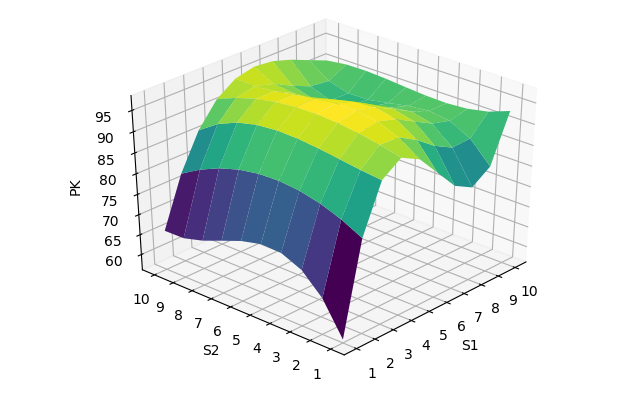
\includegraphics[width=\textwidth]{exp_3.png}
    \caption{Wykres poprawności klasyfikacji sieci dla różnej ilości neuronów}
    \label{fig:exp_3}
    % \vspace{0.5cm}
\end{figure}

Z wykresu widać, że dla małej ilości neuronów w pierwszej warstwie kiepsko się uczy. Wysokie wyniki sieć osiąga dla 5 neuronów w warstiwe pierwszej oraz 3-6 neuronów w warstwie drugiej, z najlepszym wynikiem 97\% dla $S_1=5$ i $S_2=4$.


\subsection{Wpływ współczynnika uczenia na poprawność klasyfikacji}

Następnymi badanymi wartościami są $lr_{inc}$ oraz $lr_{dec}$ czyli współczynniki decydujące o tym jak bardzo współczynnik uczenia będzie rósł lub malał w trakcie nauki. Do badania przyjęto wartości w zakresie [1.0, 1.9] dla $lr_{inc}$ oraz [0.5, 0.8] dla $lr_{dec}$. Do przeprowadzenia eksperymentu użyto poniższego kodu:

\begin{pythoncode}
a, b = np.arange(1.00, 1.91, 0.1), np.arange(0.5, 0.81, 0.05)
lr_inc, lr_dec = np.meshgrid(a, b)
result = np.empty(lr_dec.shape)

for i, row in enumerate(zip(lr_inc, lr_dec)):
    for j, params in enumerate(zip(*row)):
        learning_data, testing_data = load_wine()
        net = nn.NeuralNetwork(0.01, 100, [5, 4], 1.04, *params, 0.020)
        net.feed_training_data(*learning_data)
        net.feed_test_data(*testing_data)
        net.start_learning()
        result[i][j] = net.test(*testing_data)[2]
\end{pythoncode}

\noindent Efektem działania tego skryptu jest poniższy wykres:

\begin{figure}[h]
    \centering
    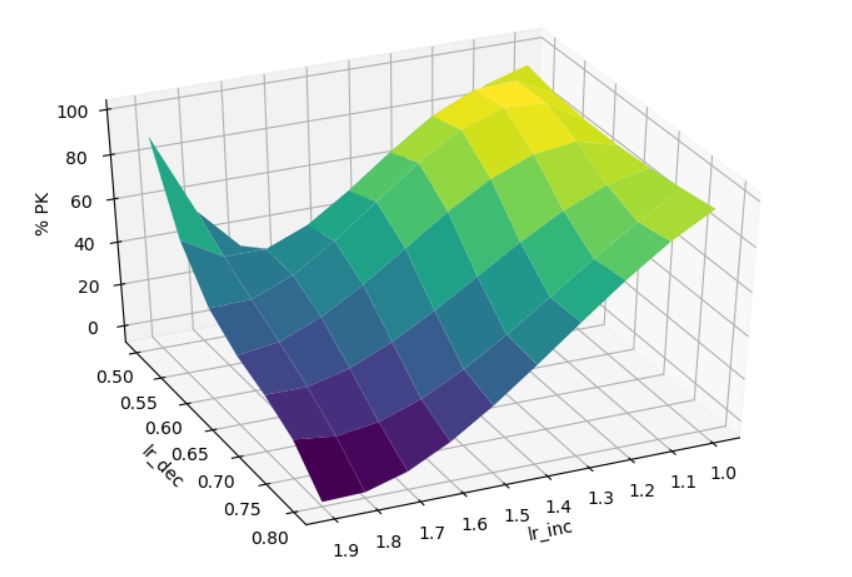
\includegraphics[width=\textwidth]{exp_4.png}
    \caption{Wykres poprawności klasyfikacji sieci dla różnej wartości współczynników $lr_{inc}$ i $lr_{dec}$}
    \label{fig:exp_4}
    % \vspace{0.5cm}
\end{figure}

Jak widać na wykresie, dla zbyt dużych $lr_{inc}$ i $lr_{dec}$ sieć traci zbieżność i nie potrafi poprawnie klasyfikować wina. Natomiast dla $lr_{inc}$ między 1.1, a 1.3 oraz $lr_{dec}$ od 0.55 do 0.60 wyniki sięgają 97\%.


\subsection{Wpływ współczynnika błędu na poprawność klasyfikacji}

W ostatnim eksperymencie ustalone zostanie jaka wartość współczynnika błędu ($err\_ratio$) najlepiej sobie radzi z wykorzystywanym zestawem danych.

\noindent Wykorzystany kod:
\begin{pythoncode}
ratios = np.arange(1.01, 1.9, 0.01)
results = np.empty((1, len(ratios)))

for i, err_ratio in enumerate(ratios):
    learning_data, testing_data = load_wine()
    net = nn.NeuralNetwork(0.01, 100, [5, 4], 1.04, 1.2, 0.6, 0.020)
    net.feed_training_data(*learning_data)
    net.feed_test_data(*testing_data)
    net.start_learning()
    pk = net.test(*testing_data)[2]
    results[j][i] = pk
\end{pythoncode}

\noindent Efekty badania przedstawia poniższy wykres:
\begin{figure}[h]
    \centering
    \begin{tikzpicture}
        \begin{axis}[
            width=\textwidth,
            height=0.5\textwidth,
            xlabel={Error ratio},
            ylabel={Poprawność klasyfikacji},
            every axis plot/.append style={ultra thick},
            ymin=0,
            % no markers,
        ]
        % \addplot table[mark=none] {data/exp_5.dat};
        \addplot table[mark=none] {data/err_ratios.csv};
        % \addplot table[mark=none] {data/err_ratios2.csv};
        \end{axis}
    \end{tikzpicture}
    
    \vspace{1cm}

    \begin{tikzpicture}
        \begin{axis}[
            width=\textwidth,
            height=0.5\textwidth,
            xlabel={Error ratio},
            ylabel={Poprawność klasyfikacji},
            every axis plot/.append style={ultra thick},
            ymin=0,
            xmax=1.3,
            % no markers,
        ]
        % \addplot table[mark=none] {data/exp_5.dat};
        \addplot table[mark=none] {data/err_ratios.csv};
        % \addplot table[mark=none] {data/err_ratios2.csv};
        \end{axis}
    \end{tikzpicture}
    \caption{Wykres poprawności klasyfikacji sieci dla poszczególnych wartości $err\_ratio$}
    \label{fig:exp_5}
    % \vspace{0.5cm}
\end{figure}

Pomimo licznych prób przeprowadzenia eksperymentu za każdym razem wyniki różniły się od siebie i nie można było jednoznacznie określić dla jakich wartości $err\_ratio$ sieć uczy się lepiej lub gorzej. Jedyną zauważoną zależnością są mniejsze wahania PK dla mniejszego \textit{error ratio}.

% \begin{figure}[h]
%     \centering
    
%     \caption{Wykres poprawności klasyfikacji sieci dla poszczególnych wartości $err\_ratio$}
%     \label{fig:exp_5}
%     % \vspace{0.5cm}
% \end{figure}

\pagebreak

\section{Wnioski}

Dzięki wykonaniu eksperymentów można było zauważyć jak bardzo różne konfiguracje parametrów sieci neuronowej wpływają na proces nauczania. W większości przypadków wyniki eksperymentów były do siebie zbliżone z wyjątkiem ostatniego eksperymentu, w którym nie udało się skorelować zmian badanego współczynnika z konkretną poprawą lub pogorszeniem procesu nauczania. 

Pierwszy eksperyment pokazał jak użycie algorytmu Nguyena-Widrowa wpływa już na pierwsze epoki uczenia. W porównaniu do sieci z losowymi wagami nauka od początku była obarczona mniejszym błędem, a wszelkie wahania kosztu odbywały się w niewielkim zakresie. Implementacja tego rozwiązania nie była skomplikowana, a rezultowała dużo lepszymi wynikami.

W drugim eksperymencie dodanie linijki odpowiedzialnej za sortowanie danych uczacych spowodowało pogorszenie się procesu nauczania. Sieć lepiej reagowała na rozlosowane dane dużo szybciej zbiegając do poprawnej klasyfikacji zadanych danych wejściowych.

Trzeci eksperyment był istotny dla tworzenia sieci ponieważ pozwolił ustalić przy jakich najmniejszych ilościach neuronów w 2 warstwach ukrytych sieć osiąga wysoki wynik poprawności klasyfikacji. Początkowe testy przesiewowe pozwoliły zawęzić przeszukiwany zakres neuronów do zakresu [1, 10], następnie właściwa część eksperymentu pozwoliła na określenie $S_1=5$ oraz $S_2=4$ jako najlepszych wartości. Dzięki temu kolejnych eksperymentów nie trzeba już było wykonywać na większych warstwach, przy których sieć być może osiągnęłaby podobne wyniki lecz przy dłuższym czasie uczenia.

W przypadku współczynnika zmniejszania oraz zwiększania współczynnika uczenia ustalono, że najlepsze wyniki sieć otrzymuje dla $lr_{dec} \approx 0.6$ oraz $lr_{inc} \approx 1.2$.

Wyniki ostatniego eksperymentu niestety nie były wystarczająco jednoznaczne przez co nie udało się ustalić czy wykorzystywany $err\_ratio=1.04$ był wartością odpowiednią. Pomimo wielokrotnych prób otrzymywane dane różniły się od siebie i nie pozwalały na zauważenie konkretnej tendencji spadkowej lub wzrostowej.


\pagebreak
\begin{thebibliography}{9}
    \addcontentsline{toc}{section}{Literatura}

    \bibitem{dataset} S. Aeberhard, \emph{Wine Data Set}, UCI - Machine Learning Repository, 1991.\\\href{http://archive.ics.uci.edu/ml/datasets/wine}{http://archive.ics.uci.edu/ml/datasets/wine}
    \bibitem{zajdel_6} R. Zajdel, \emph{Sztuczna inteligencja, Laboratorium, Ćwiczenie 6 Model neuronu}, PRz, KIiA, Rzeszów.
    \bibitem{sigmoid_derivative} M. Percy, \emph{Derivative of sigmoid function $\sigma(x)=\frac{1}{1+e^{-x}}$}, 2017.\\\href{https://math.stackexchange.com/a/1225116}{https://math.stackexchange.com/a/1225116}
    \bibitem{book_osowski} S. Osowski, \emph{Sieci neuronowe do przetwarzania informacji}, Oficyna Wydawnicza Politechniki Warszawskiej, Warszawa 2006.
    \bibitem{book_rutkowski} L. Rutkowski, \emph{Metody i techniki sztucznej inteligencji}, Wydawnictwo Naukowe PWN, Warszawa, 2009.
    \bibitem{mathworks_adaptive} MathWorks Inc., \emph{Gradient descent with adaptive learning rate backpropagation - MATLAB traingda}\\\href{https://www.mathworks.com/help/deeplearning/ref/traingda.html}{https://www.mathworks.com/help/deeplearning/ref/traingda.html}
    \bibitem{initnw} \emph{NeuroLab 0.3.5 documentation}\\\href{https://pythonhosted.org/neurolab/_modules/neurolab/init.html}{https://pythonhosted.org/neurolab/\_modules/neurolab/init.html}
    \bibitem{nguyen_widrow} D. Nguyen, B. Widrow, \emph{Improving the Learning Speed of 2-Layer Neural Networks by Choosing Initial Values of the Adaptive Weights}, Stanford University, 1990, Stanford
    \bibitem{zajdel_9} R. Zajdel, \emph{Sztuczna inteligencja, Laboratorium, Ćwiczenie 6 Sieć Jednokierunkowa Wielowarstwowa}, PRz, KIiA, Rzeszów.
\end{thebibliography}

\end{document}